 %%%%%%%%%%%%%%%%%%%%%%%%%%%%%%%%%%%%%%%%%
% University Assignment Title Page 
% LaTeX Template
% Version 1.0 (27/12/12)
%
% This template has been downloaded from:
% http://www.LaTeXTemplates.com
%
% Original author:
% WikiBooks (http://en.wikibooks.org/wiki/LaTeX/Title_Creation)
%
% License:
% CC BY-NC-SA 3.0 (http://creativecommons.org/licenses/by-nc-sa/3.0/)
% 
% Instructions for using this template:
% This title page is capable of being compiled as is. This is not useful for 
% including it in another document. To do this, you have two options: 
%
% 1) Copy/paste everything between \begin{document} and \end{document} 
% starting at \begin{titlepage} and paste this into another LaTeX file where you 
% want your title page.
% OR
% 2) Remove everything outside the \begin{titlepage} and \end{titlepage} and 
% move this file to the same directory as the LaTeX file you wish to add it to. 
% Then add \documentclass[12pt]{article}
\usepackage[english]{babel}
\usepackage{amsmath}
\usepackage{graphicx}
\usepackage{textcomp}
\usepackage{parskip}
\usepackage[colorinlistoftodos]{todonotes}
\usepackage{csquotes}
\usepackage{float}
\usepackage[backend=biber,style=ieee]{biblatex}
\addbibresource{bibliography.bib}

\begin{document}

\begin{titlepage}

\newcommand{\HRule}{\rule{\linewidth}{0.5mm}}
\center 

\textsc{\LARGE Iowa State University }\\[1.5cm] 
\textsc{\Large Center for Statistics and Applications in Forensic
Evidence
}\\[0.5cm] 

\HRule \\[0.4cm]
{ \huge \bfseries Shoe Print Data Collection: Additional Methods }\\[0.4cm] 
\HRule \\[1.5cm]



\begin{center}
\centering
 
\includegraphics[scale=.4]{csafe-logo}\\[1cm]
\end{center}







\end{titlepage}

\section{Introduction}

 When developing the methodology for the longitudinal shoe study conducted by the Center for Statistics and Applications in Forensic Evidence (CSAFE), collection procedures were designed to obtain the most ideal shoe-sole impression possible. While these images will be useful to the researcher and practitioner communities, they do not provide realistic examples of prints that would be collected from a crime scene/suspected crime scene. For this reason, CSAFE researchers have compiled this manual which contains procedures for further data collection and offers new, or edited, procedures that better represent the practices of current forensic examiners and crime scene teams. If at any time there is a question on any of these procedures, please make a note using a post-it note and e-mail the principal investigator, the project manager, the faculty in charge of the study, or the author of the specific procedure. 

\end{document} to your LaTeX file where you want your
% title page.
%
%%%%%%%%%%%%%%%%%%%%%%%%%%%%%%%%%%%%%%%%%
%\title{Description of Outsole Impression Methods}
%----------------------------------------------------------------------------------------
%	PACKAGES AND OTHER DOCUMENT CONFIGURATIONS
%----------------------------------------------------------------------------------------

\documentclass[12pt]{article}
\usepackage[english]{babel}
\usepackage[utf8x]{inputenc}
\usepackage{amsmath}
\usepackage{graphicx}
\usepackage[colorinlistoftodos]{todonotes}

%% Forcing images to stay in their corresponding section
\usepackage{placeins}
\let\Oldsection\section
\renewcommand{\section}{\FloatBarrier\Oldsection}
\let\Oldsubsection\subsection
\renewcommand{\subsection}{\FloatBarrier\Oldsubsection}
\let\Oldsubsubsection\subsubsection
\renewcommand{\subsubsection}{\FloatBarrier\Oldsubsubsection}


% Set images path
\graphicspath{ {images/} }

% Links to sections.
\usepackage{hyperref}

\begin{document}

\begin{titlepage}

\newcommand{\HRule}{\rule{\linewidth}{0.5mm}} % Defines a new command for the horizontal lines, change thickness here

\center % Center everything on the page
 
%----------------------------------------------------------------------------------------
%	HEADING SECTIONS
%----------------------------------------------------------------------------------------
\textsc{\LARGE Iowa State University}\\[1.5cm] % Name of your university/college
\textsc{\large Center for Statistics and Applications in Forensic Evidence }\\[0.5cm] % Minor heading such as course title

%----------------------------------------------------------------------------------------
%	TITLE SECTION
%----------------------------------------------------------------------------------------

\HRule \\[0.4cm]
{ \huge \bfseries Methods and Techniques for Shoe Sole Data Collection}\\[0.4cm] % Title of your document
\HRule \\[1.5cm]
 
%----------------------------------------------------------------------------------------
%	AUTHOR SECTION
%----------------------------------------------------------------------------------------
\begin{minipage}{0.4\textwidth}
\begin{flushleft} \large
\emph{Author:}\\
James \textsc{E. Kruse} % Your name
\end{flushleft}
\end{minipage}
~
\begin{minipage}{0.4\textwidth}
\begin{flushright} \large
\emph{Principal Investigator:} \\
Dr. Guillermo \textsc{Basulto-Elias} % Supervisor's Name
\end{flushright}
\end{minipage}\\[2cm]

% If you don't want a supervisor, uncomment the two lines below and remove the section above
%\Large \emph{Author:}\\
%John \textsc{Smith}\\[3cm] % Your name
%----------------------------------------------------------------------------------------
%	LOGO SECTION
%----------------------------------------------------------------------------------------


\includegraphics[scale=.5]{Logo}\\[1cm]

\begin{center}
\begin{tabular}{ c   |   c } 
 
\end{tabular}
\end{center}
%----------------------------------------------------------------------------------------
%	DATE SECTION
%----------------------------------------------------------------------------------------

{\large \today}\\[2cm] % Date, change the \today to a set date if you want to be precise


 
%----------------------------------------------------------------------------------------

\vfill % Fill the rest of the page with whitespace

\end{titlepage}
 
\tableofcontents

\newpage

\section{Introduction}

The objective of this document is to list, explain, and provide details on the collection methods currently being used in the ongoing shoe sole study being conducted by CSAFE. The following pages will include explanations and images of each of the 7 collection methods. Also included are examples and the reasoning behind each method.  

  This is a component of the large scale and ongoing study that is looking to develop a statistical model that could be used by forensic criminalists when identifying shoe prints. 
 

\section{Methods}
\label{sec:examples}
\subsection{Mat Scanner}

   When participants arrived to collect their shoes for the first time, they were asked to step on a Mat scanner. This scanner is a product of Tekscan and allows us to collect a sample of both the way each participant steps and the points of the foot where the most pressure is placed. 
   
   The area in which the scanner is located has spike tape marking the exact location of the device and a path leading both toward it and away. This is to limit the variability in approach and also to make communicating directions to the participants easier. 
   
   Participants themselves walk 6 times across the mat per foot. Half of these are wearing nothing but a thin disposable sock on the foot and the other half are wearing their shoe, or a new shoe of the same type. Each scan is then saved as a video, 2 different CSV files, and as a jpg image. 

\begin{figure}[!htp]
\centering
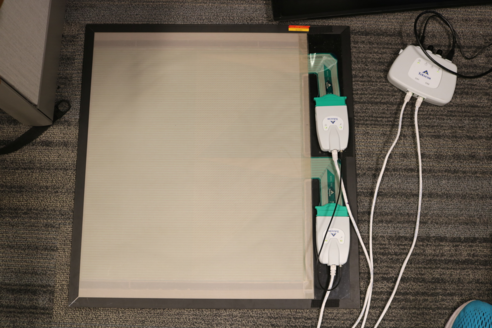
\includegraphics[width=12cm, height=8cm]{Mat_Scanner}
\caption{Mat Scanner}
\label{Image 1}
\end{figure}

\begin{figure}[!htp]
\centering
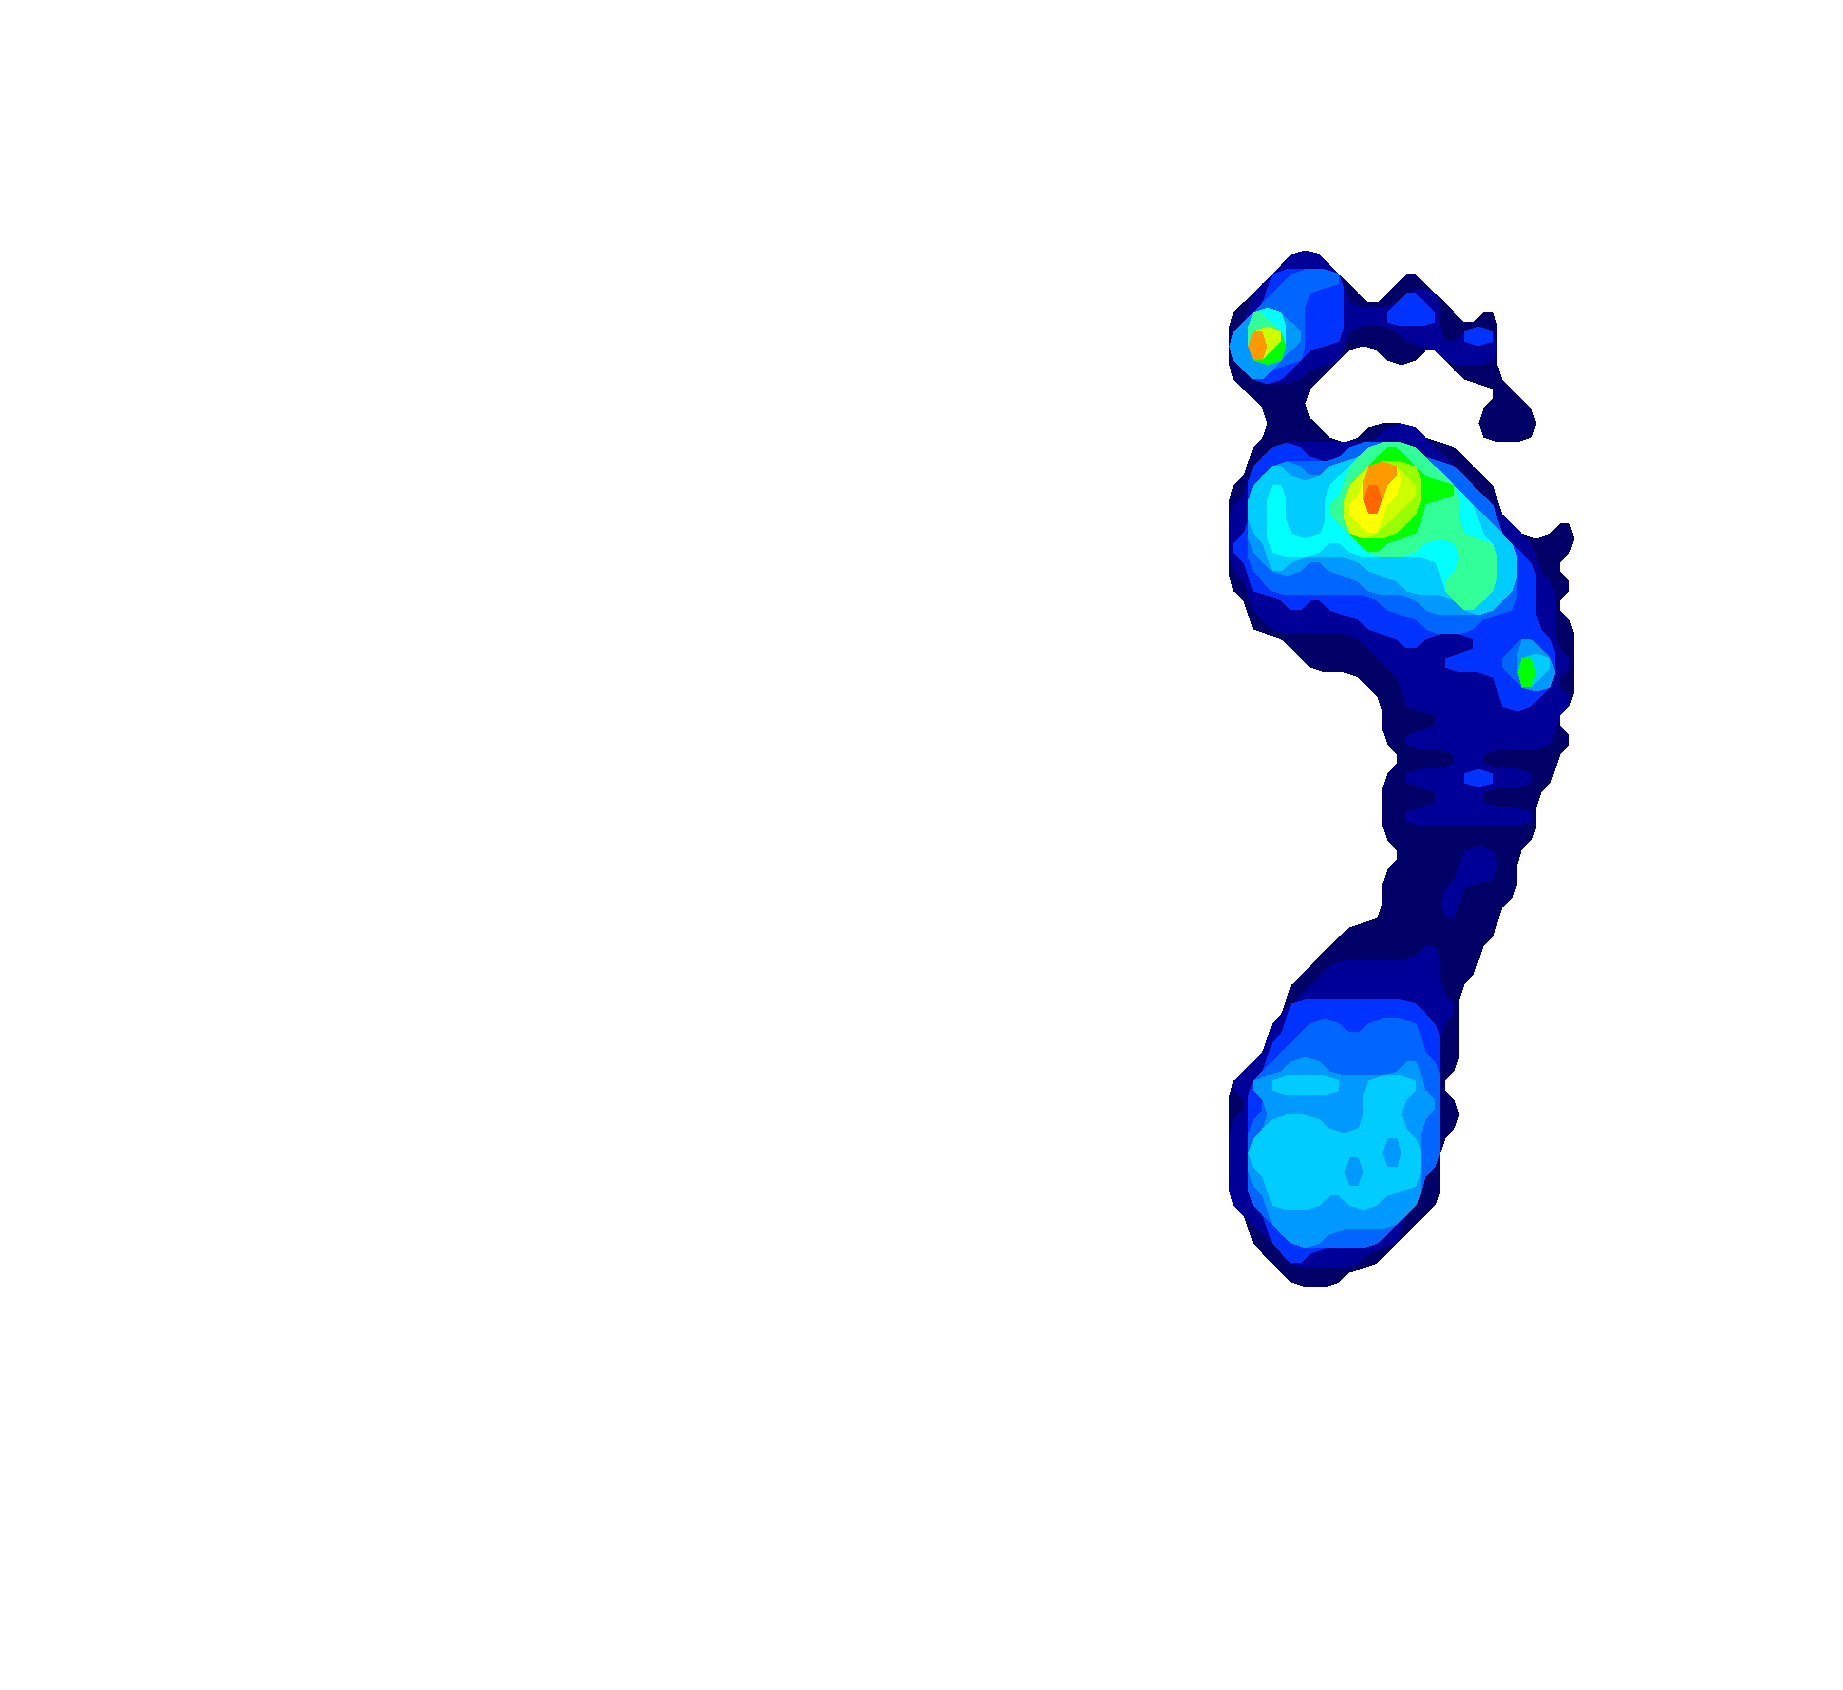
\includegraphics[scale=0.2]{Mat_Foot}
\caption{Foot jpg}
\label{Image 2}
\end{figure}

\begin{figure}[!htp]
\centering
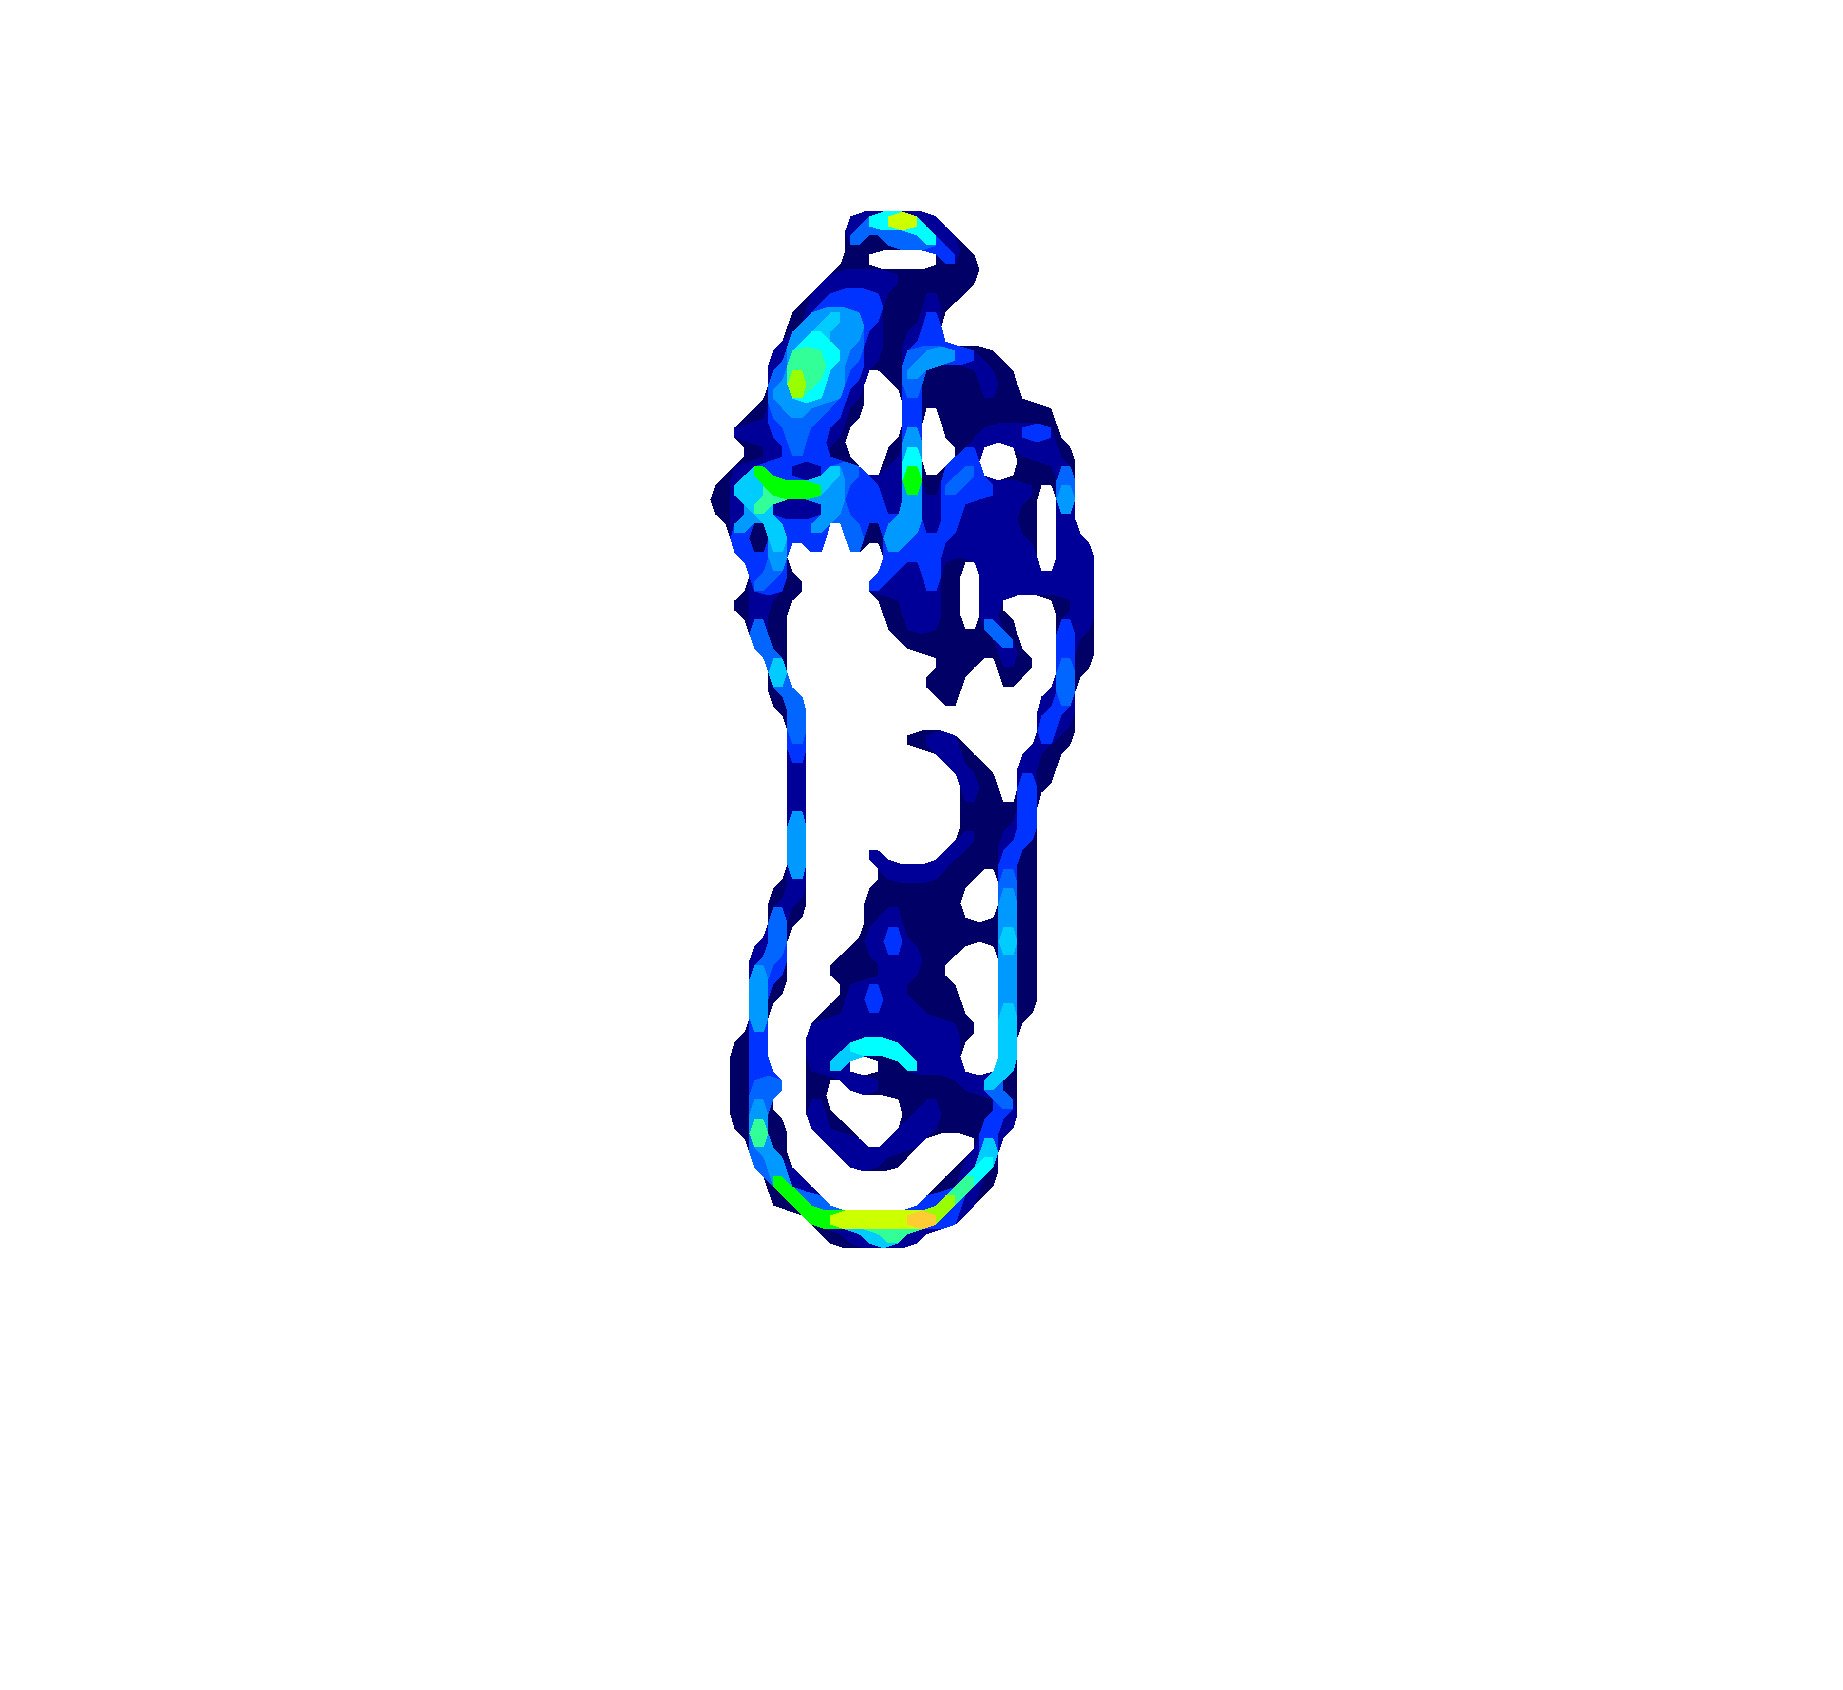
\includegraphics[scale=0.2]{Mat_shoe}
\caption{Adidas jpg}
\label{Image 3}
\end{figure}

\subsection{High Definition Photography}

   The first method of data collection to be used at each delivery is high definition photography. A Cannon camera is set up on a tripod. Below the lens, the shoe is set into a box that keeps it stable. Next to the shoe, a ruler on a stand is set up for scale. The tag from the bag is set next to it so that the date and shoe number can be seen in the final image. 
   
   The camera is hooked up to a laptop so that at no time does the research technician need to touch the camera itself. Two images are captured and saved for each shoe. 
   
   These photos are being taken as both a reference to what the shoe looks like when new or when coming in for a periodic collection and for their possible assistance with the end goal. 

\begin{figure}[!htp]
\centering
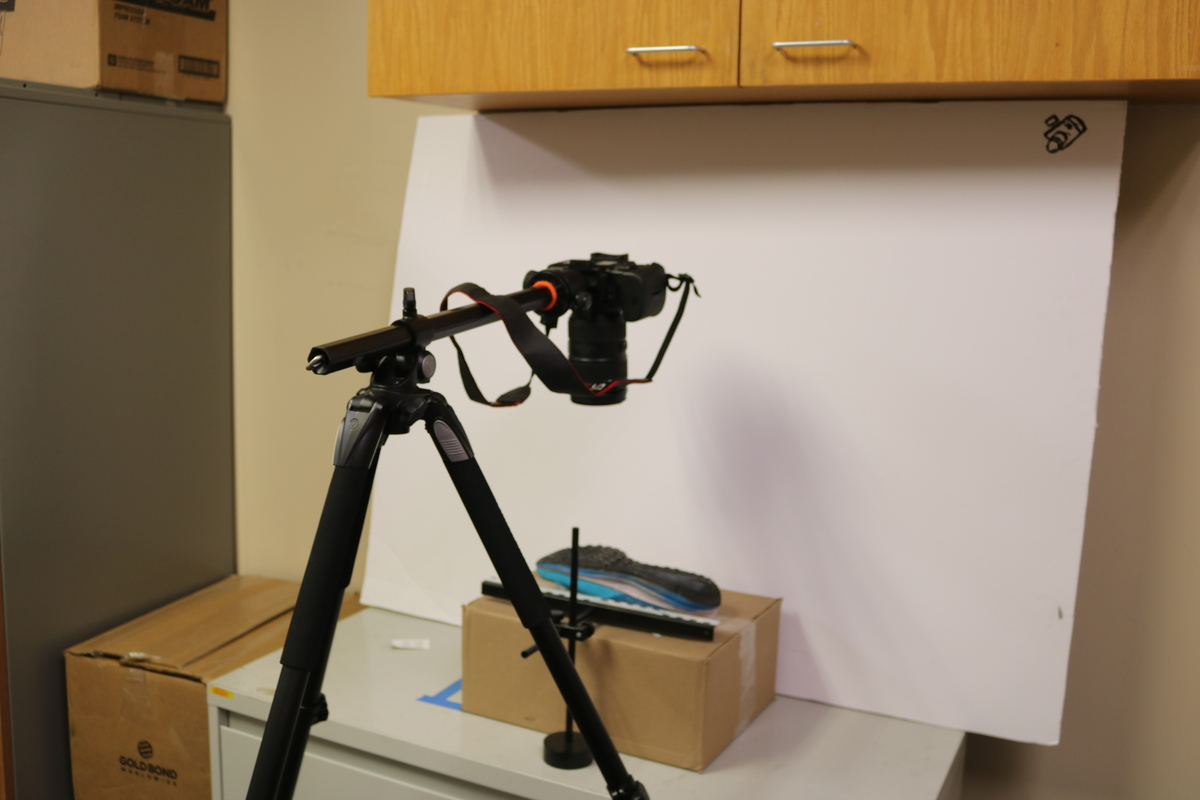
\includegraphics[width=12cm, height=8cm]{Original_Camera_Set}
\caption{Full camera set up}
\label{Image 4}
\end{figure}

\begin{figure}[!htp]
\centering
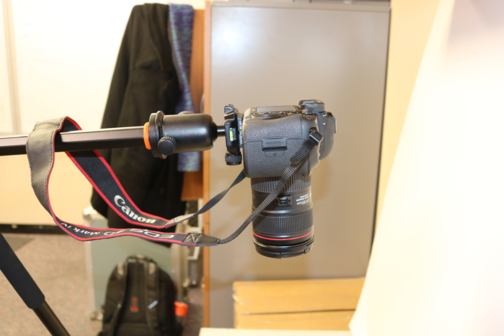
\includegraphics[width=12cm, height=8cm]{Camera}
\caption{Cannon Camera}
\label{Image 5}
\end{figure}

\begin{figure}[!htp]
\centering
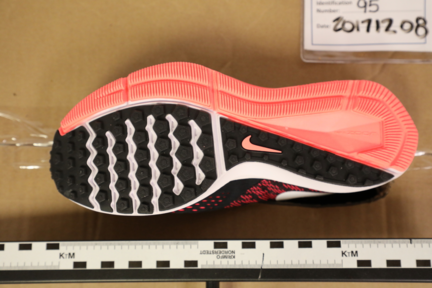
\includegraphics[width=12cm, height=8cm]{Baseline_Photo}
\caption{Adidas}
\label{Image 6}
\end{figure}



\subsection{Everspry 2D Shoe Sole Scans}

   The second method of data collection being utilized during this study is 2D digital scanning. An Everspry 2D scanner is hooked up to a computer that has had the software for the device downloaded. The subject then puts on the shoe to be scanned and walks across the scanner. 
   
   For the purposes of this study, two walking methods are being used when taking scans. For each shoe, the first two prints are detailed scans. The subject points their toe towards the ceiling and places their heel on the scanner. Carefully, they then step down and shift their foot within the shoe. The goal of this method is to get a clear scan with as much detail as possible. 
   
   The second method involved is the taking of a walking print. The subject walks up to the scanner and then steps onto the scanner. Immediately after, they step off as if walking down a road. These four images are then saved as STL files. 

   This method provides researchers with a clean and easy to work with digital image of the shoe sole. 
   
\begin{figure}[!htp]
 \centering
 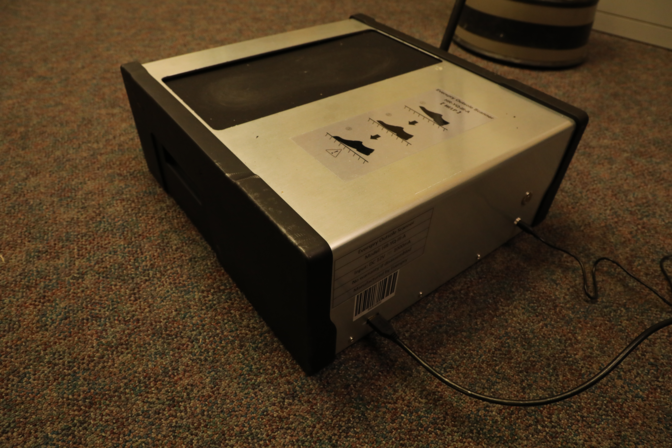
\includegraphics[width=12cm]{2D_Scanner}
 \caption{2D Scanner }
 \label{Image 7}
\end{figure}

\begin{figure}[!htp]
\centering
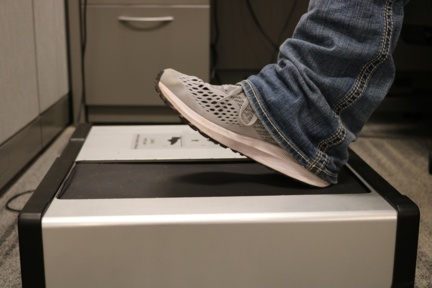
\includegraphics[width=12cm]{2D_Step_on}
\caption{Stepping on the Scanner}
\label{Image 8}
\end{figure}

\begin{figure}[!htp]
\centering
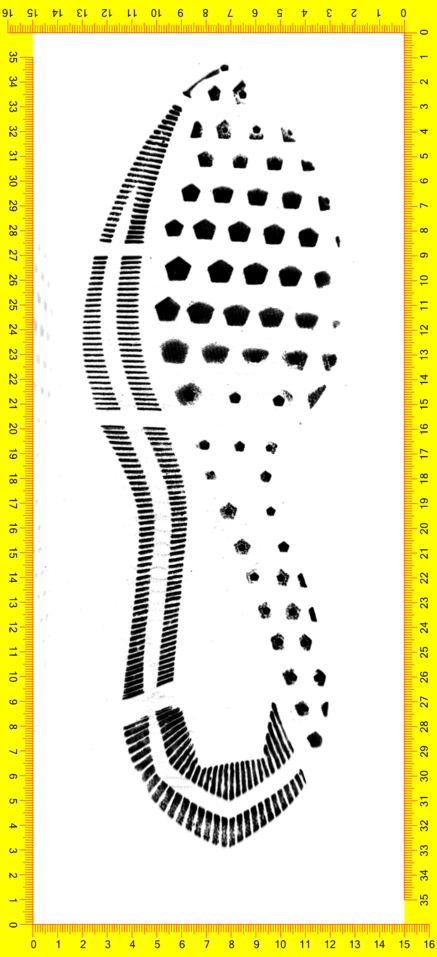
\includegraphics[width=5cm]{2D_1}
\caption{Sample 2D Scan}
\label{Image 9}
\end{figure}


\subsection{3D shoe Sole Scans}

   The third method of data collection being utilized for this study is 3D shoe sole scanning. The devise used is an EinScan-Pro+ hand held 3D scanner that connects directly to a computer. Once the software is installed, it allows technicians to take high quality scans of shoe soles. 
   
   The shoe is placed on a stand which orients the sole toward the technician. The scanner is then turned on and slowly moved back and forth across the shoe. The image can be seen coming together on the computer screen. After a rough image has been compiled, the technician should adjust the brightness of the scan. This allows the image to gain more detail. 
   
   This method, like the 2D scanner, provides researchers with a manageable and clean digital 3D replicate of the shoe sole. These are easy to work with and provide more detail then can be seen in other scans. 
   
   \begin{figure}[!htp]
\centering
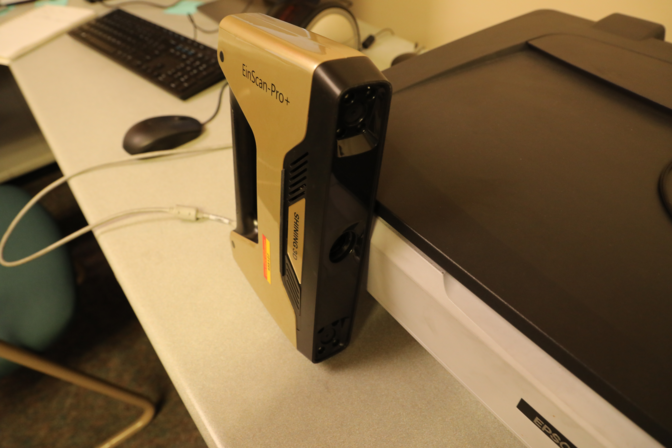
\includegraphics[width=12cm]{3D_Scanner}
\caption{3D Scanner}
\label{Image 10}
\end{figure}

\begin{figure}[!htp]
\centering
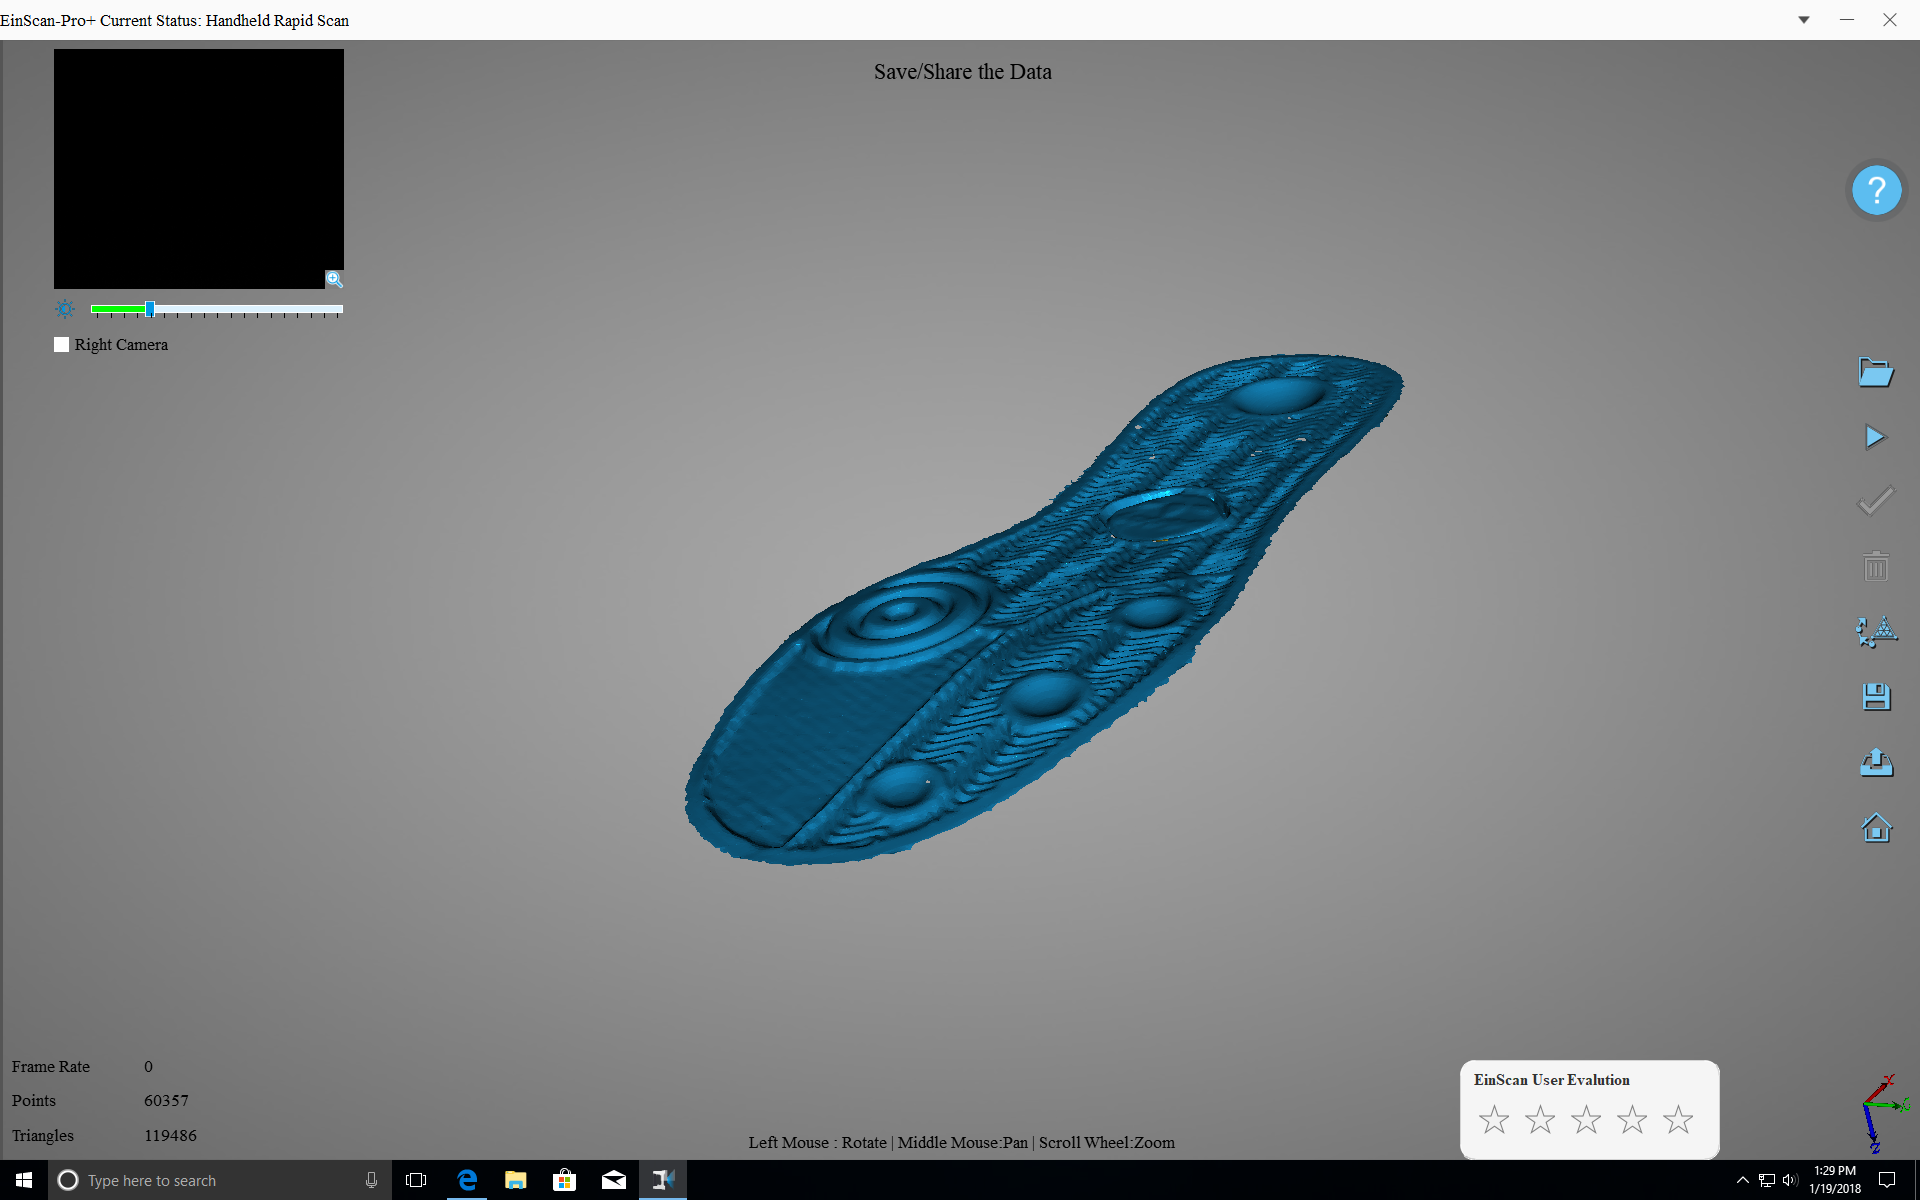
\includegraphics[width=12cm]{3D_Adidas}
\caption{Sample 3D scan}
\label{Image 11}
\end{figure}

\begin{figure}[!htp]
\centering
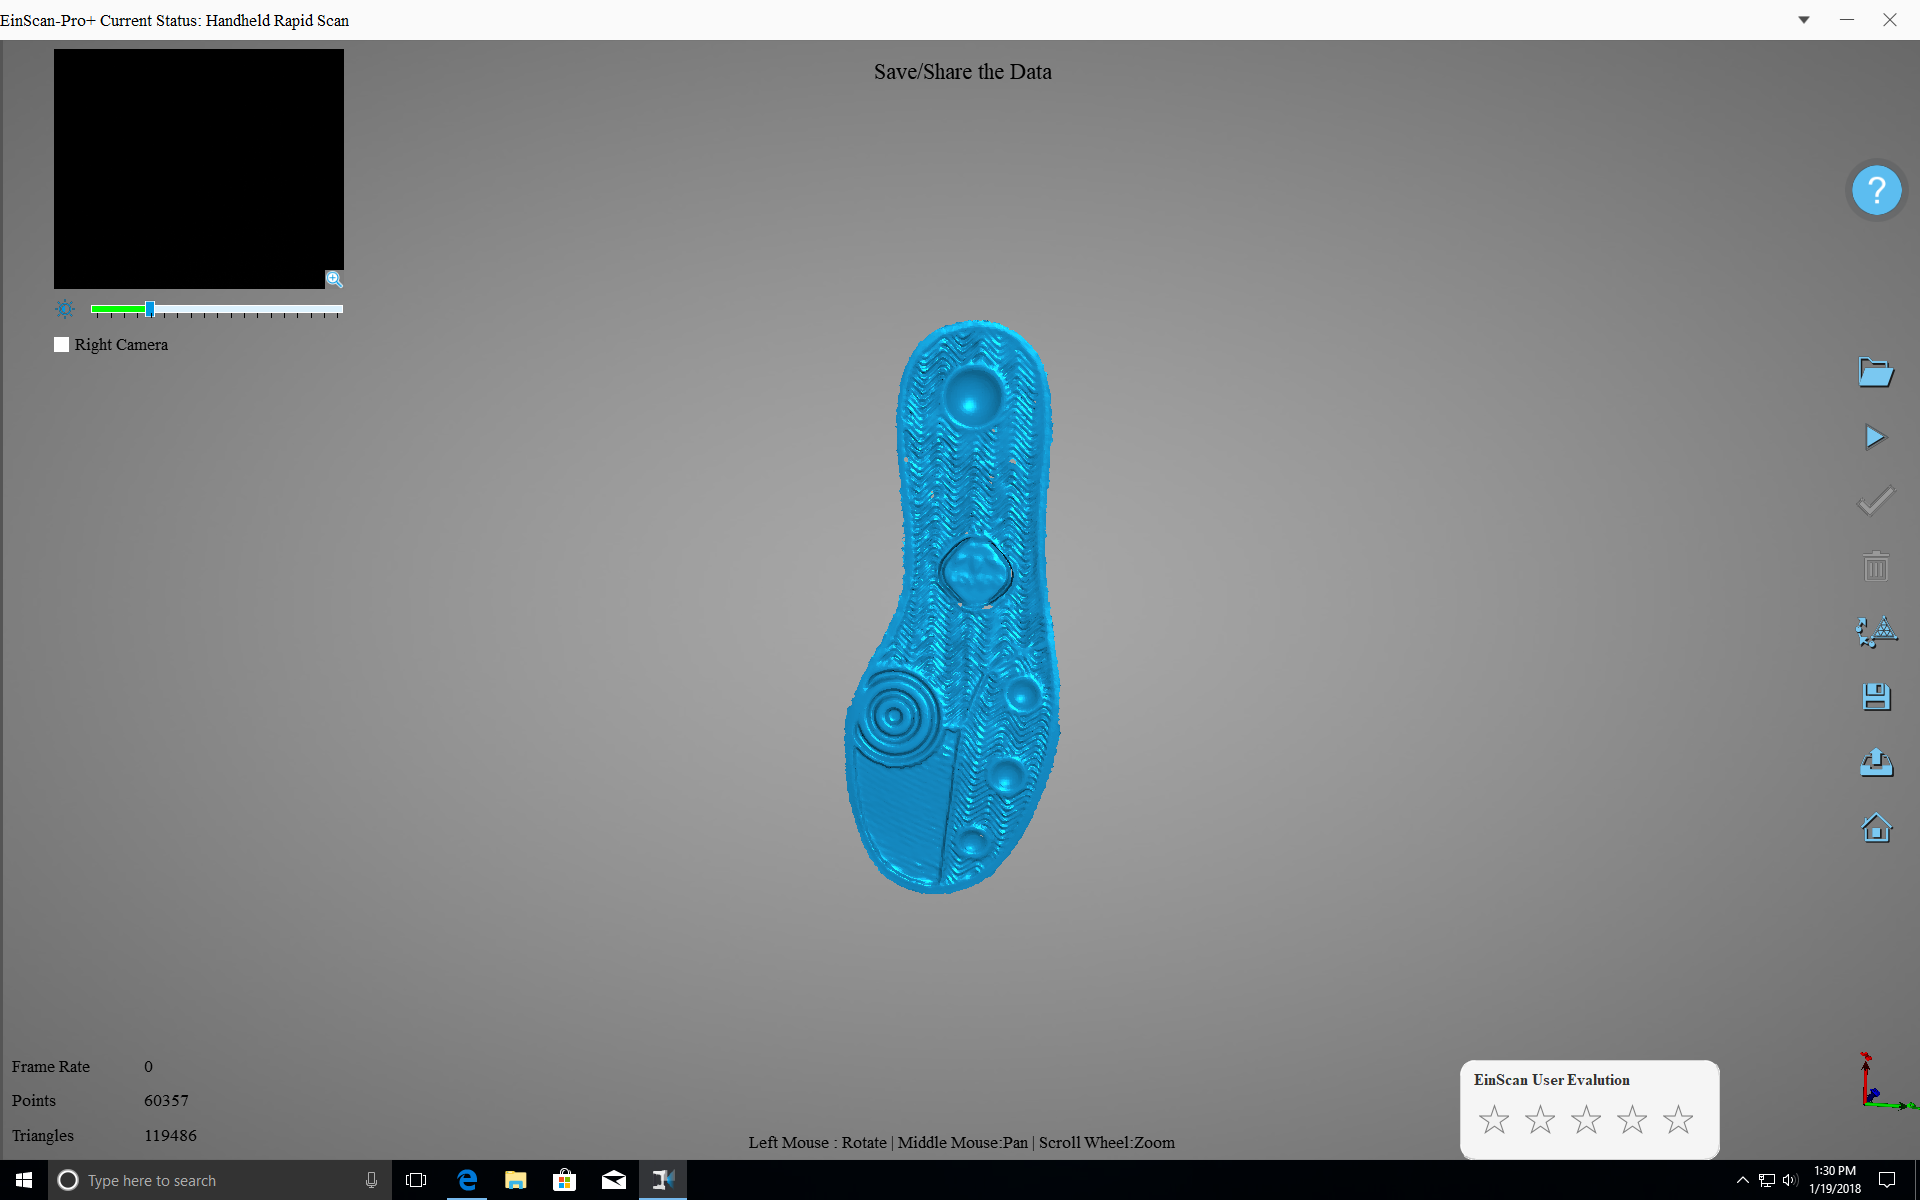
\includegraphics[width=12cm]{3D_Adidas_2}
\caption{Sample 3D Scan}
\label{Image 12}
\end{figure}


\subsection{Powder Film Prints}

   The fourth method being utilized for this study is film powder prints. This method involves using clear sticky films to take powder prints of the shoe soles. Two different types of film prints are taken, but the shoes must only be brushed once per set. 
   
   The shoe soles are brushed with silver finger print powder using a brush also meant for finger printing. Compressed air, held roughly 7 inches away, is then passed over the shoe soles in order to get rid of any excess dust. The shoe is then set aside and the other shoe in the pair can then be powdered. 
   
   On the ground, newspaper is laid out and a chair is pulled up next to it. While the subject puts on one of the shoes, without touching the sole, the technician removes the clear film from its back. The film is placed on the newspaper in front of the subject. Guiding the subjects shoe down onto the film, the subjects place their heel on the film with their toe pointing towards the ceiling. They then roll their foot into a flat standing position and step up so that all of their weight is on the film. Weight is shifted in the shoe in order to capture all detail possible. 

   While the technician is holding the back corners (by the heel) of the film, carefully the subject steps off of the film. Peeling the foot forward until only the tip of the toe is making contact with the adhesive. At this point, they step straight off, but do not place the powdered shoe on the ground. The back is then carefully replaced on the film and a label is placed on the back. 


   For the second print, place the clear portion, sticky side facing up, on the news paper near the subject. Guide the subjects shoe down onto the paper. The subject should place their heel on the film with their toe pointing towards the ceiling. They will then roll their foot into a flat standing position and step up so that all of their weight is on the film. They will then lift their foot, with the film attached, so that the sole is facing the technician. At this point, the technician will manually press all portions of the film into the shoe, making sure to get all grooves and indents if possible. After the film has been thoroughly pressed in, the technician will remove the film. The subject is now free to walk on the shoe. 
   
   These prints have the ability to take on smaller details then the digital prints. 
   
\begin{figure}[!htp]
\centering
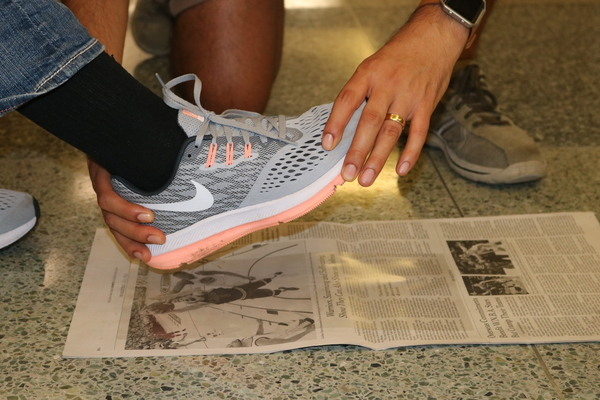
\includegraphics[width=12cm]{Film_Place}
\caption{Taking a film print}
\label{Image 13}
\end{figure}

\begin{figure}[!htp]
\centering
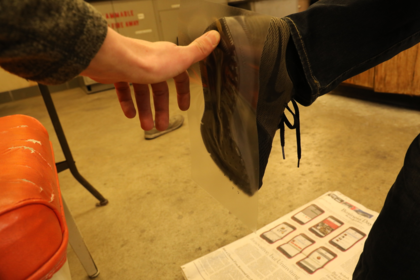
\includegraphics[width=12cm]{Press}
\caption{Taking a detail film print}
\label{Image 14}
\end{figure}

\begin{figure}[!htp]
\centering
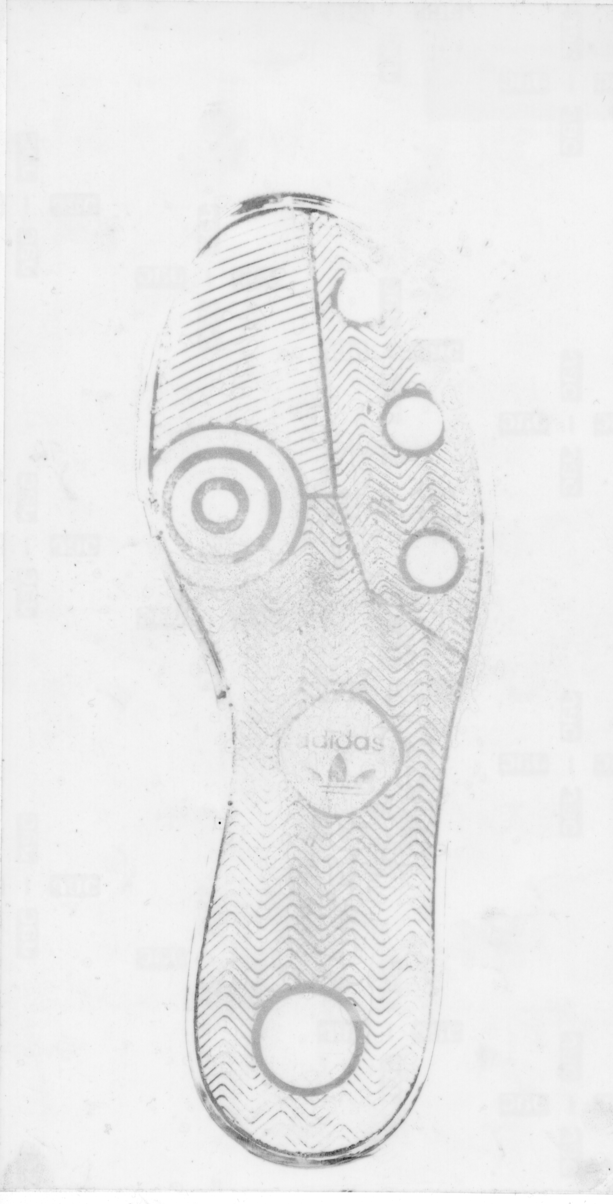
\includegraphics[width=5cm]{Film_1_Baseline}
\caption{Film Print}
\label{Image 15}
\end{figure}

\begin{figure}[!htp]
\centering
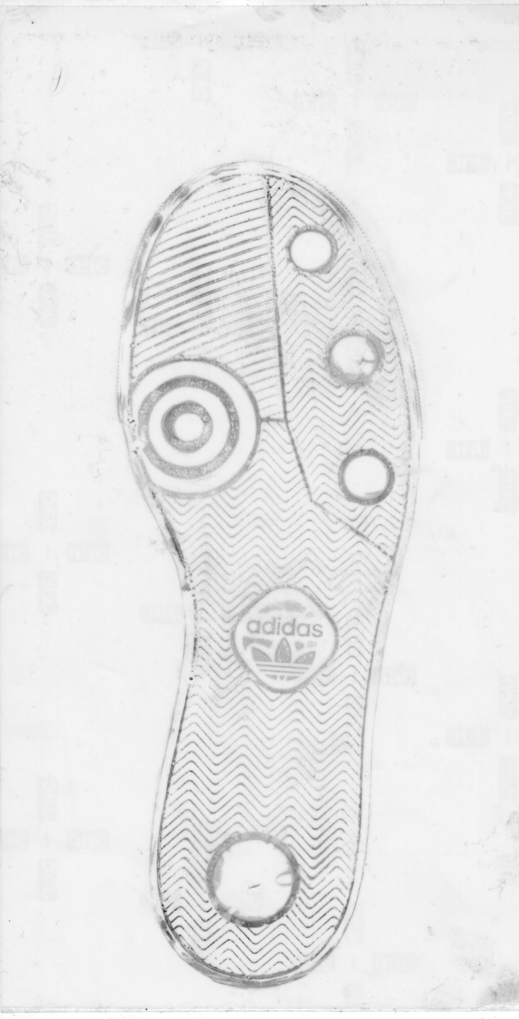
\includegraphics[width=5cm]{Film_2_Baseline}
\caption{Detail Film Print}
\label{Image 16}
\end{figure}


\subsection{Paper Powder Prints}

   The fifth method being utilized for this study is paper-powder printing. This method involves using 4 legal size pieces of printer paper to collect shoe prints that have been made with black powder. Each shoe will generate 5 prints, but the shoes must only be brushed once per set. 
   
     The shoe soles are brushed with black finger print powder using a brush also meant for finger printing. Compressed air, held roughly 7 inches away, is then passed over the shoe soles in order to get rid of any excess dust. The shoe is then set aside and the other shoe in the pair can then be powdered. 
    
   A trail of 4 pieces of paper are laid end to end in front of the subject, who is sitting on a chair. The subject must put on a powdered shoe without touching the sole. The technician then guides the subjects shoe down onto the paper. The subject should place their heel on the lower portion of the paper with their toe pointing towards the ceiling. They will then roll their foot into a flat standing position and step up so that all of their weight is concentrated at one point. The subject will shift their weight in the shoe in order to capture all detail possible. 

  At this point, the subject will step straight off, but not place the powdered shoe on the ground. On the second paper, they position the foot in the same way, but take a step as if walking normally. Again, they do not place the powdered shoe on the ground. On the third paper, the subject stamps their foot straight down. At this point, they step straight off, but do not place the powdered shoe on the ground. On the fourth paper, the subject steps and slightly twists to smudge the print. Then step straight off, but do not place the powdered shoe on the ground Lastly, the subject walks across the vinyl flooring that way laid at the end in the same way that they did for the second sheet of paper. 

   The completed prints are then labeled and laminated in order to protect the print.The vinyl flooring pieces are labeled and set aside for later use. 
   
   These prints do not come out perfect. They are meant to simulate prints that would be found at a crime scene. 
   
\begin{figure}[!htp]
\centering
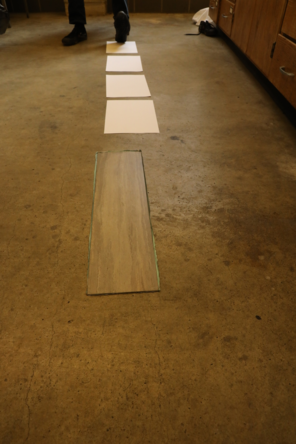
\includegraphics[width=12cm, angle=-90]{Path}
\caption{Paper print set up}
\label{Image 17}
\end{figure}

\begin{figure}[!htp]
\centering
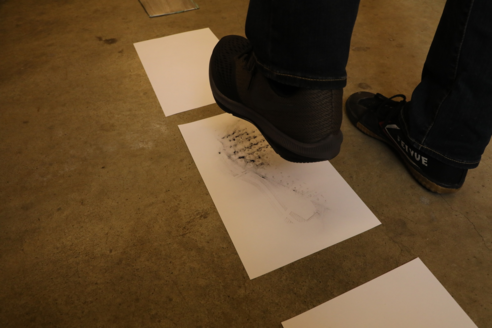
\includegraphics[width=12cm]{Stomp}
\caption{Taking paper print 3}
\label{Image 18}
\end{figure}

\begin{figure}[!htp]
\centering
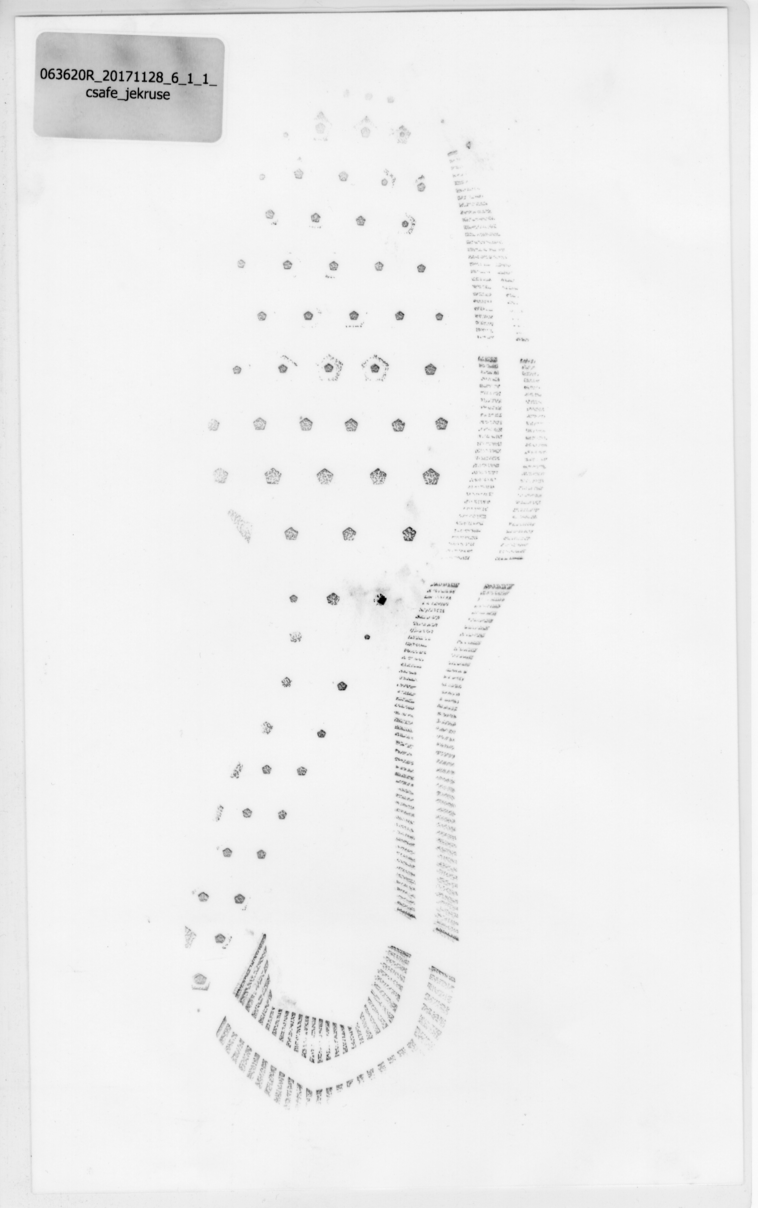
\includegraphics[width=5cm]{Baseline_Paper_1}
\caption{Paper print 1}
\label{Image 19}
\end{figure}

\begin{figure}[!htp]
\centering
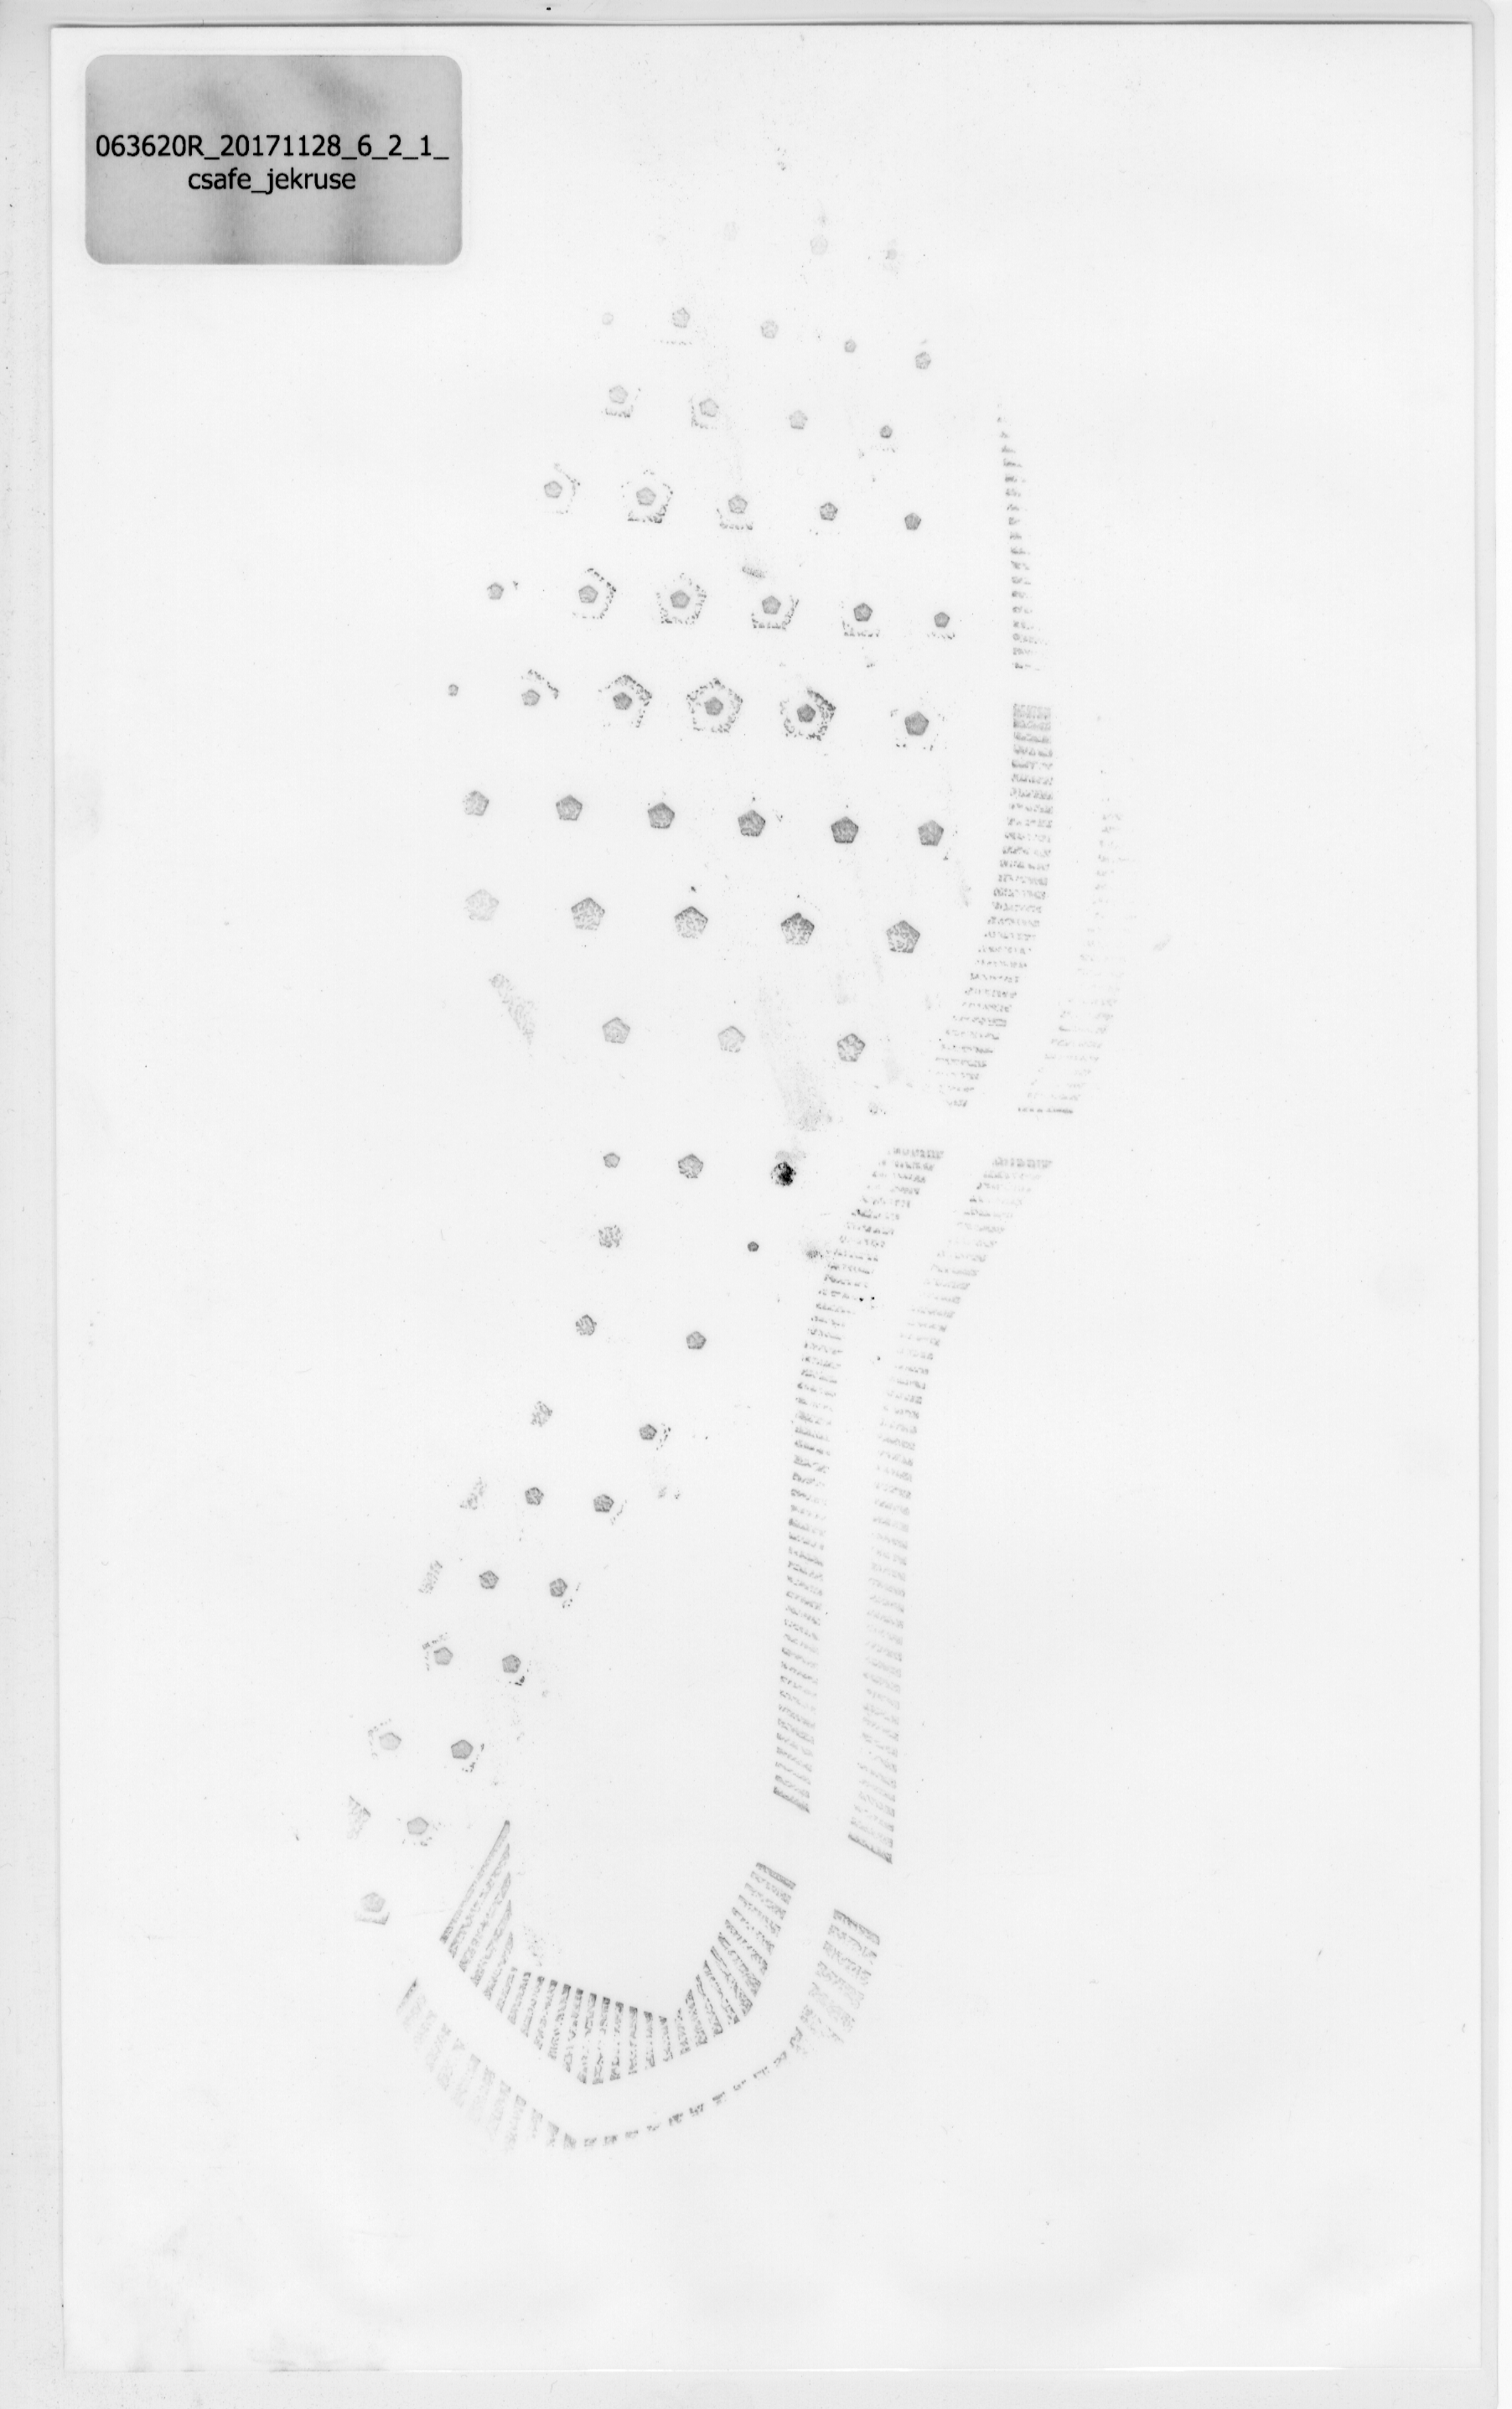
\includegraphics[width=5cm]{Baseline_Paper_2}
\caption{Paper print 2}
\label{Image 20}
\end{figure}

\begin{figure}[!htp]
\centering
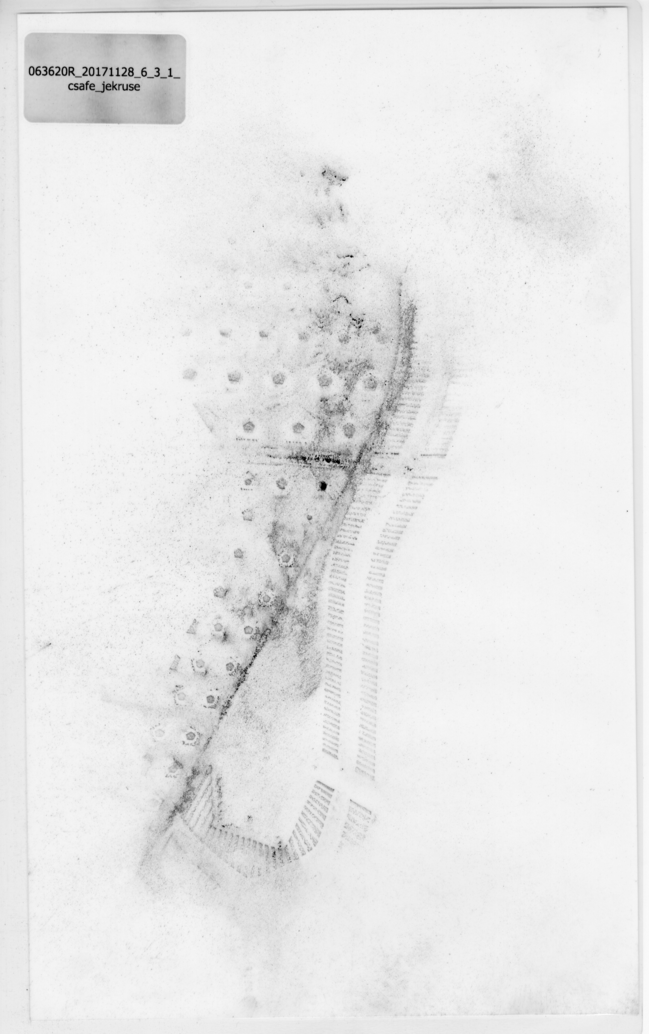
\includegraphics[width=5cm]{Baseline_Paper_3}
\caption{Paper print 3}
\label{Image 21}
\end{figure}

\begin{figure}[!htp]
\centering
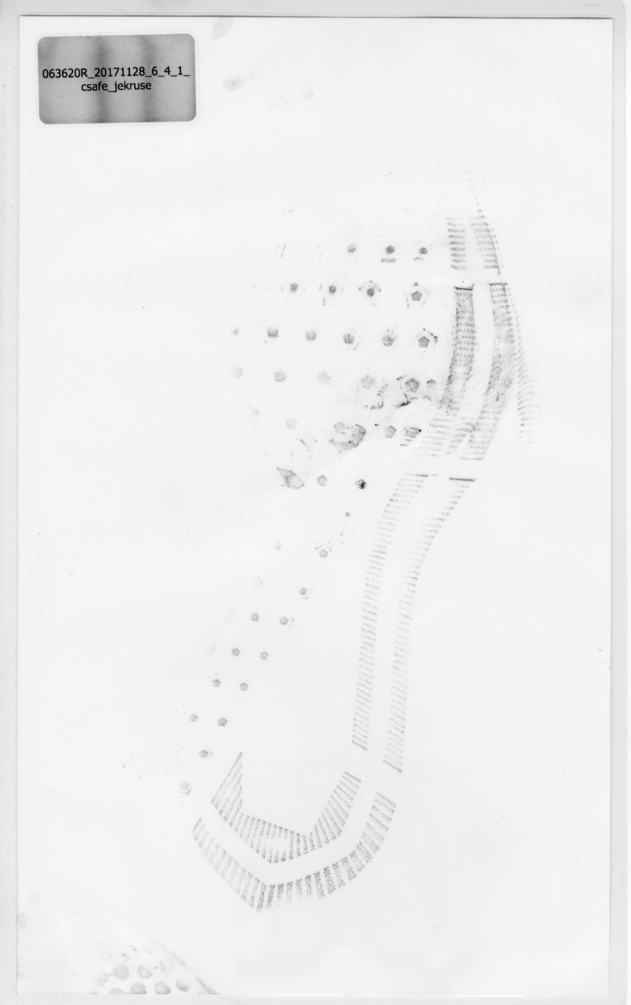
\includegraphics[width=5cm]{Baseline_Paper_4}
\caption{Paper print 4}
\label{Image 22}
\end{figure}

\subsection{Vinyl Prints}

   The sixth and final method being utilized for this study is vinyl flooring prints.These pints were taken during the paper-print procedure, but are prepossessed at a different time.
   
   In the marked off area, the technician will position the flooring and the lights on the pre-laid spike tape. A ruler will be positioned next to the vinyl for scale. They will then turn off the light, computer monitors, and shut the door. This will make sure that light does not effect the photos.

   Standing overhead of the print, the technician will take a photo straight down as if at a crime scene. The camera should be zoomed in on the full print even if the toe or heel is not completely visible. The lights should be positioned as they are in the example images (do not use the flash. (Note: the label written in dry erase marker must be visible in the photo.) 

   For the second rep., the tech will alter the name written in marker to account for the second image making sure not to damage the print. They will take a second photo using the same procedure as above. 

   Once all photos have been taken, the vinyls are completely cleaned and allowed to dry. The images themselves are meant to simulate a print that was obtained from a household floor. 

\begin{figure}[!htp]
\centering
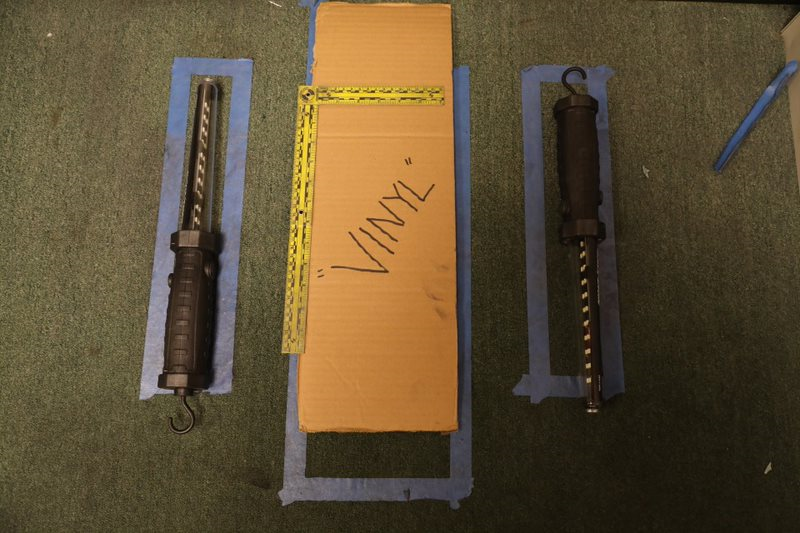
\includegraphics[width=12cm]{Baseline_Vinyl_set}
\caption{Vinyl Set Up}
\label{Image 23}
\end{figure}

\begin{figure}[!htp]
\centering
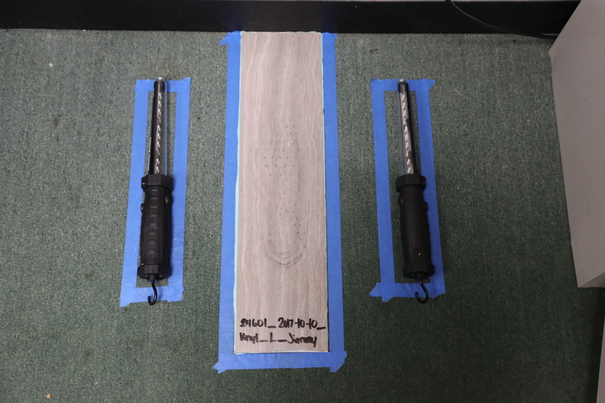
\includegraphics[width=12cm]{vinyl_set}
\caption{Vinyl prints being taken}
\label{Image 24}
\end{figure}

\begin{figure}[!htp]
\centering
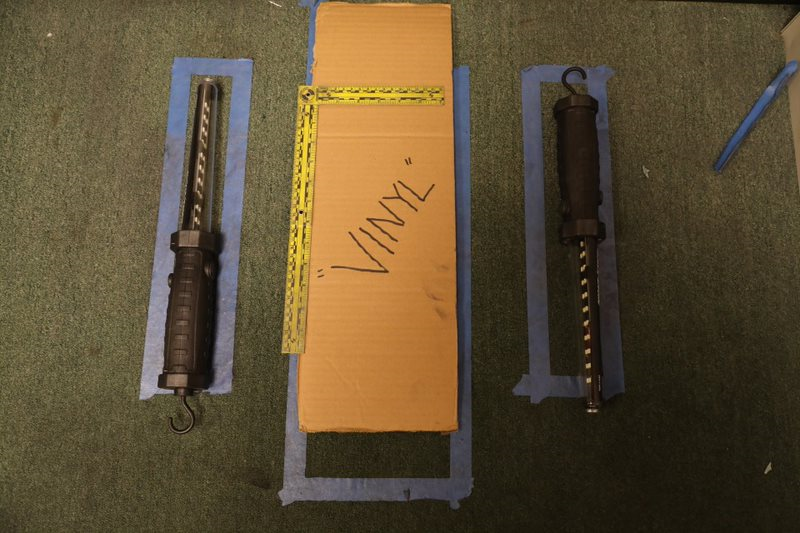
\includegraphics[width=18cm, angle=90]{Baseline_Vinyl_set}
\caption{Vinyl prints being taken}
\label{Image 25}
\end{figure}

\end{document}

